\chapter{Metodologia} \label{metodologia}

O Capítulo~\ref{RevisaoBibliografica} apresentou a revisão bibliográfica, neste capítulo sera apresentada a metodologia do trabalho. Na Figura~\ref{fig:quadro} pode-se ver um detalhamento do projeto.

\begin{figure}[ht] % ht para here, b para     bottom e t para top
    \begin{center}
    \caption{Descrição da legenda.} %//não esqueça o ponto final
    \label{fig:quadro}
    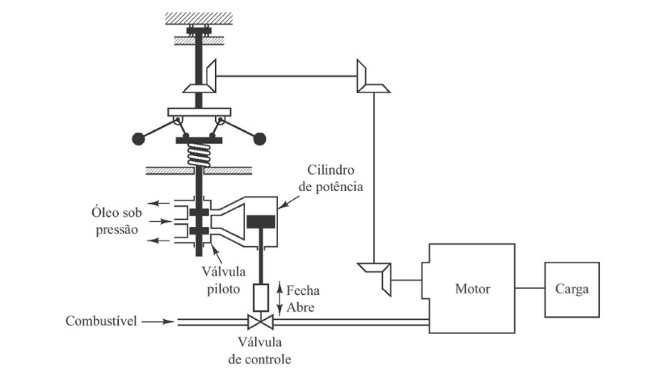
\includegraphics[width=0.9\linewidth]{Figuras/imagem1.JPG} \\
    \end{center}
    \fonte{\citeauthor{ogata}, \citeyear{ogata}. }    
\end{figure}

A Figura~\ref{fig:icone} é uma figura elaborado pelo autor em 2020. Veja como fica a legenda.

\begin{figure}[H] % ht para here, b para     bottom e t para top
    \begin{center}
    \caption{Imagem do autor.} %//não esqueça o ponto final
    \label{fig:icone}
    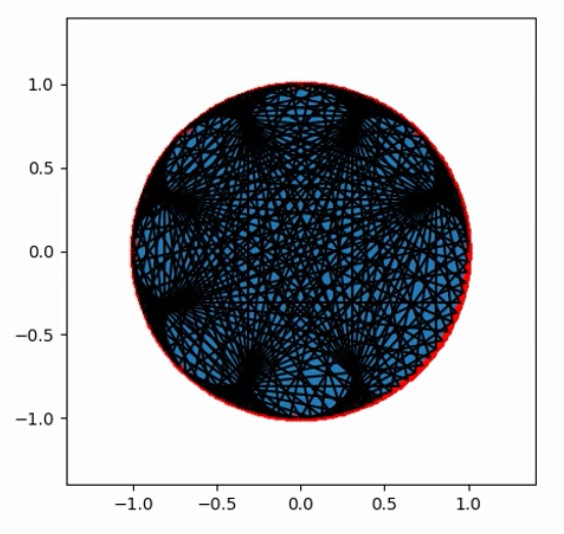
\includegraphics[width=0.5\linewidth]{Figuras/imagem2.jpg} \\
    \end{center}
    \fonteautor
    %\fontsize{10}{12}\selectfont{Fonte: Elaborado pelo autor, \imprimirano. }
    
\end{figure}


A Figura~\ref{fig:ifmg} é uma figura retirada de um site.

\begin{figure}[H] % h! para here, b para bottom e t para top
   \begin{center}
    \caption{Logo do IF SUDESTE MG - Campus Muriaé.} %//não esqueça o ponto final
    \label{fig:ifmg}
    
\includegraphics[width=0.5\linewidth]{Figuras/logoifsudestemg.png} \\
    \end{center}    
    \fonte{\href{https://www.ifsudestemg.edu.br/muriae}{https://www.ifsudestemg.edu.br/muriae}.}    
    
\end{figure}

%\par\bigskip % acrescenta um espaço para forçar o texto ser depois da imagem

\dangersign[5ex]  {\color{red}
Obs.: Siga os exemplos deste capítulo sempre que for inserir uma nova figura!
}


O formulário utilizado na pesquisa pode ser encontrado no ANEXO~\ref{anexoA}.

Exemplo de quadro, conforme Quadro~\ref{qd:exemplo}.

\begin{quadro}[htb]
  \centering
  \caption{Exemplo de quadro.}\label{qd:exemplo}
  \begin{tabular}{cp{12cm}}
    \hline \hline &\\[-0.4cm]
    \textbf{Etapas} & \textbf{Descrição} \\
    \hline
    &\\[-0.4cm]
    \textbf{1} & Leitura das regras. \\[0.2cm]
    \textbf{2} & Revisão da literatura de trabalhos correlacionados. \\[0.2cm]
    \textbf{3}& Implementação.\\[0.2cm]
    \textbf{4} & Validação. \\[0.2cm]
    \textbf{5} & Produção científica e/ou documentação.\\[0.2cm]
    \hline \hline
  \end{tabular}
\end{quadro}


Exemplo de cronograma, conforme Tabela~\ref{tb:cronograma}.

\begin{table}[!ht]
     \caption{Cronograma do projeto.}\label{tb:cronograma}
	\centering
	\resizebox{\linewidth}{!}{
		\begin{tabular}{|c|c|c|c|c|c|c|c|c|c|c|c|c|} \hline
		& \multicolumn{12}{c|}{Meses}\\ \cline{2-13}
         \raisebox{1.5ex}{Etapas} & 01 & 02 & 03 & 04 & 05 & 06 & 07 & 08 & 09 & 10 & 11 & 12 \\		\hline
		1&\cellcolor{midgray}&\cellcolor{midgray}&\cellcolor{midgray}&\cellcolor{midgray}&&&&&\cellcolor{midgray}&\cellcolor{midgray}&\cellcolor{midgray}&\\
		\hline
		2&&&\cellcolor{midgray}&\cellcolor{midgray}&\cellcolor{midgray}&&&&&&&\\
		\hline	
		3&&&&\cellcolor{midgray}&\cellcolor{midgray}&\cellcolor{midgray}&&&&&&\\
		\hline			
		4&&&&\cellcolor{midgray}&\cellcolor{midgray}&\cellcolor{midgray}&\cellcolor{midgray}&&&&&\\
		\hline	
		5&&&&&&&&\cellcolor{midgray}&\cellcolor{midgray}&&&\\
		\hline
		
		
		\end{tabular}
		}
\end{table}

\clearpage
